\section{MER}

\subsection{Decisiones de Dise�o}

\begin{enumerate}
	\item Ruta es d�bil en relaci�n a un recorrido porque s�lo sirve como una forma de ir desde el origen del recorrido a su destino.
	\item Contingencia es una entidad d�bil porque puede haber una cantidad arbitraria de ellas por cada viaje realizado(en contraposici�n a una lista de contingencias predefinidas ej:choque, bloqueo de ruta, control policial, etc) y las mismas no tienen sentido sin su viaje relacionado.
	\item La ruta tiene asociado un clima por cada periodo del a�o. Como se menciono en las hipotesis el periodo son las estaciones del a�o.\\ Para ello contamos con tres entidades: ruta, clima y estaci�n. Estas tres siempres est�n vinculadas juntas. Es decir, para cada (ruta,clima) existe una instancia de estaci�n, por cada (clima, estaci�n) se vincula a una ruta y por cada par (ruta, estacion) hay un clima asociado. Por tal motivo es que decidimos modelarlo como una ternaria.
	\item Con lo que respecta al chofer y la licencia, nos pareci� m�s acorde separarlas en dos entidad pese a que en los requerimientos no queda clara dicha separaci�n. Lo realizamos as� para mayor claridad.
	\item Con respecto al dise�o de la entidad \textbf{Direcci�n} primero se opt� por hacerla d�bil de la ciudad.			
	
\begin{center}
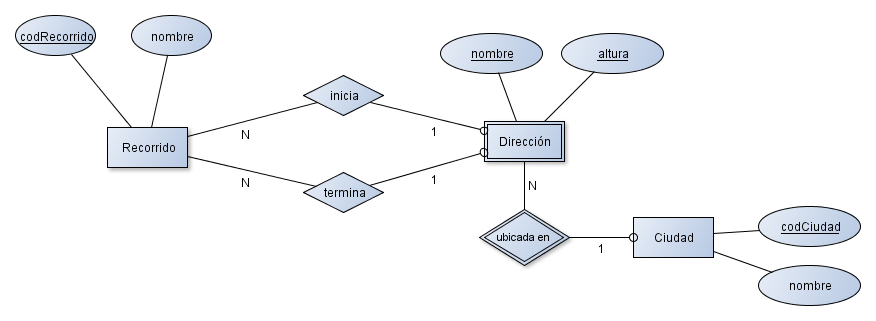
\includegraphics[scale=0.50]{img/RecorridoDirDebil.png}
\end{center}

Al poner como clave primaria de \textbf{Direccion} su altura y nombre junto a la clave primaria de la ciudad, propag�bamos estas tres claves como for�neas en otras entidad vinculadas.

Luego optamos por dejar \textbf{Direcci�n} como una entidad fuerte con una clave primaria \textbf{codDir} para as� evitar la propagaci�n de claves y obtener un dise�o m�s sencillo.

\begin{center}
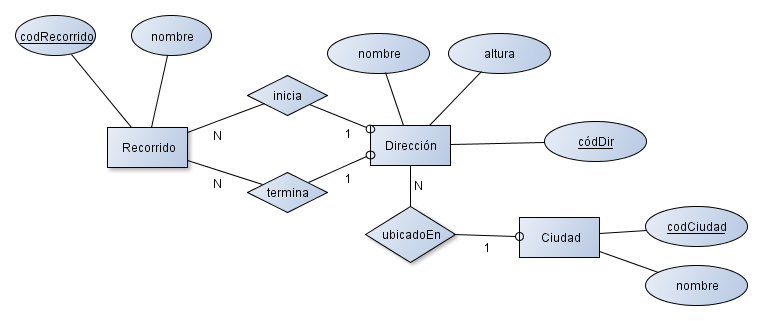
\includegraphics[scale=0.50]{img/RecorridoDirFuerte.png}
\end{center}

Vale aclarar que este dise�o admite tuplas duplicados con el mismo codDir, altura, nombre y c�digo de ciudad, sin embargo podemos impedir dicha situaci�n agregando una restricci�n adicional al DER.
  
\item Decidimos no guardar la historia de las reparaciones. Hubieramos podido hacerla de esta manera.

\begin{center}
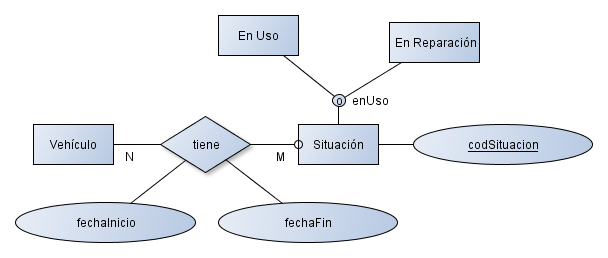
\includegraphics[scale=0.50]{img/ReparacionConHistoria.png}
\end{center}

En este dise�o hubieramos necesitado agregar restricciones para asegurar que para toda fecha posterior a $Vehiculo.fechaAlta$ el $Vehiculo$ debe tener \textbf{solo y exactamente una} $Situacion$

Pero como no hay requerimientos expl�citos por los cuales necesitemos guardar la historia, decidimos simplificar el dise�o de la siguiente manera:

\begin{center}
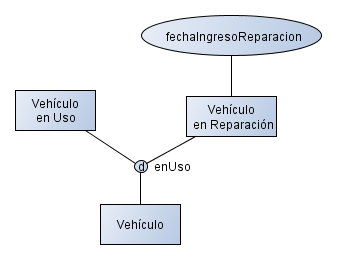
\includegraphics[scale=0.50]{img/ReparacionSinHistoria.png}
\end{center}

\item Consideramos originalmente particionar los viajes en planificados y realizados, como se muestra en el siguiente diagrama:

\begin{center}
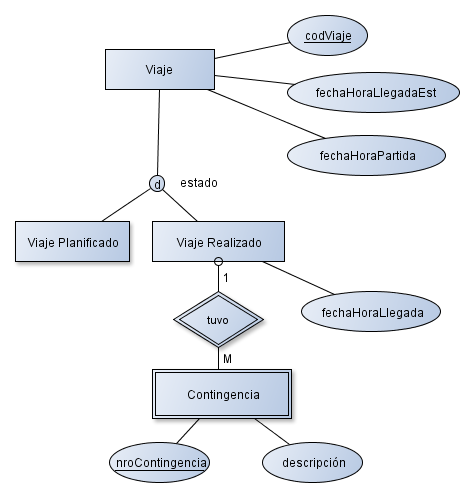
\includegraphics[scale=0.50]{img/viajePlanificado-Realizado.png}
\end{center}

Nos pareci� mejor considerar los viajes realizados como una especializaci�n de los planificados(todos los viajes son planificados y algunos de ellos adem�s pueden ser realizados). Esto lo dise�amos como una relaci�n de overlapping con una sola entidad llamada \textbf{Viaje Realizado}, describiendo que todos los viajes realizados heredan los mismos atributos que un viaje planificado, pero solo algunos viajes planificados tienen su correspondiente realizado.

\begin{center}
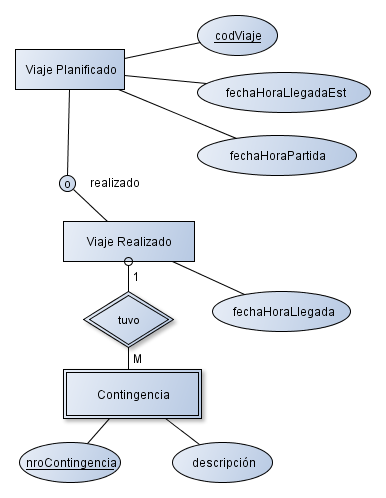
\includegraphics[scale=0.55]{img/viaje-Planificado-Realizado.png}
\end{center}

\item $(Chofer/Viaje Planificado)/Control$ es una agregaci�n pues no toda relacion $Chofer/Viaje Planificado$ tiene controles asociados.
Adem�s $Control$ es una Entidad asociada a la interrelacion entra $Vaje Planificado$ y $Control$ y no a una de ellas en particular.

\end{enumerate}

\subsection{DER}

\begin{center}
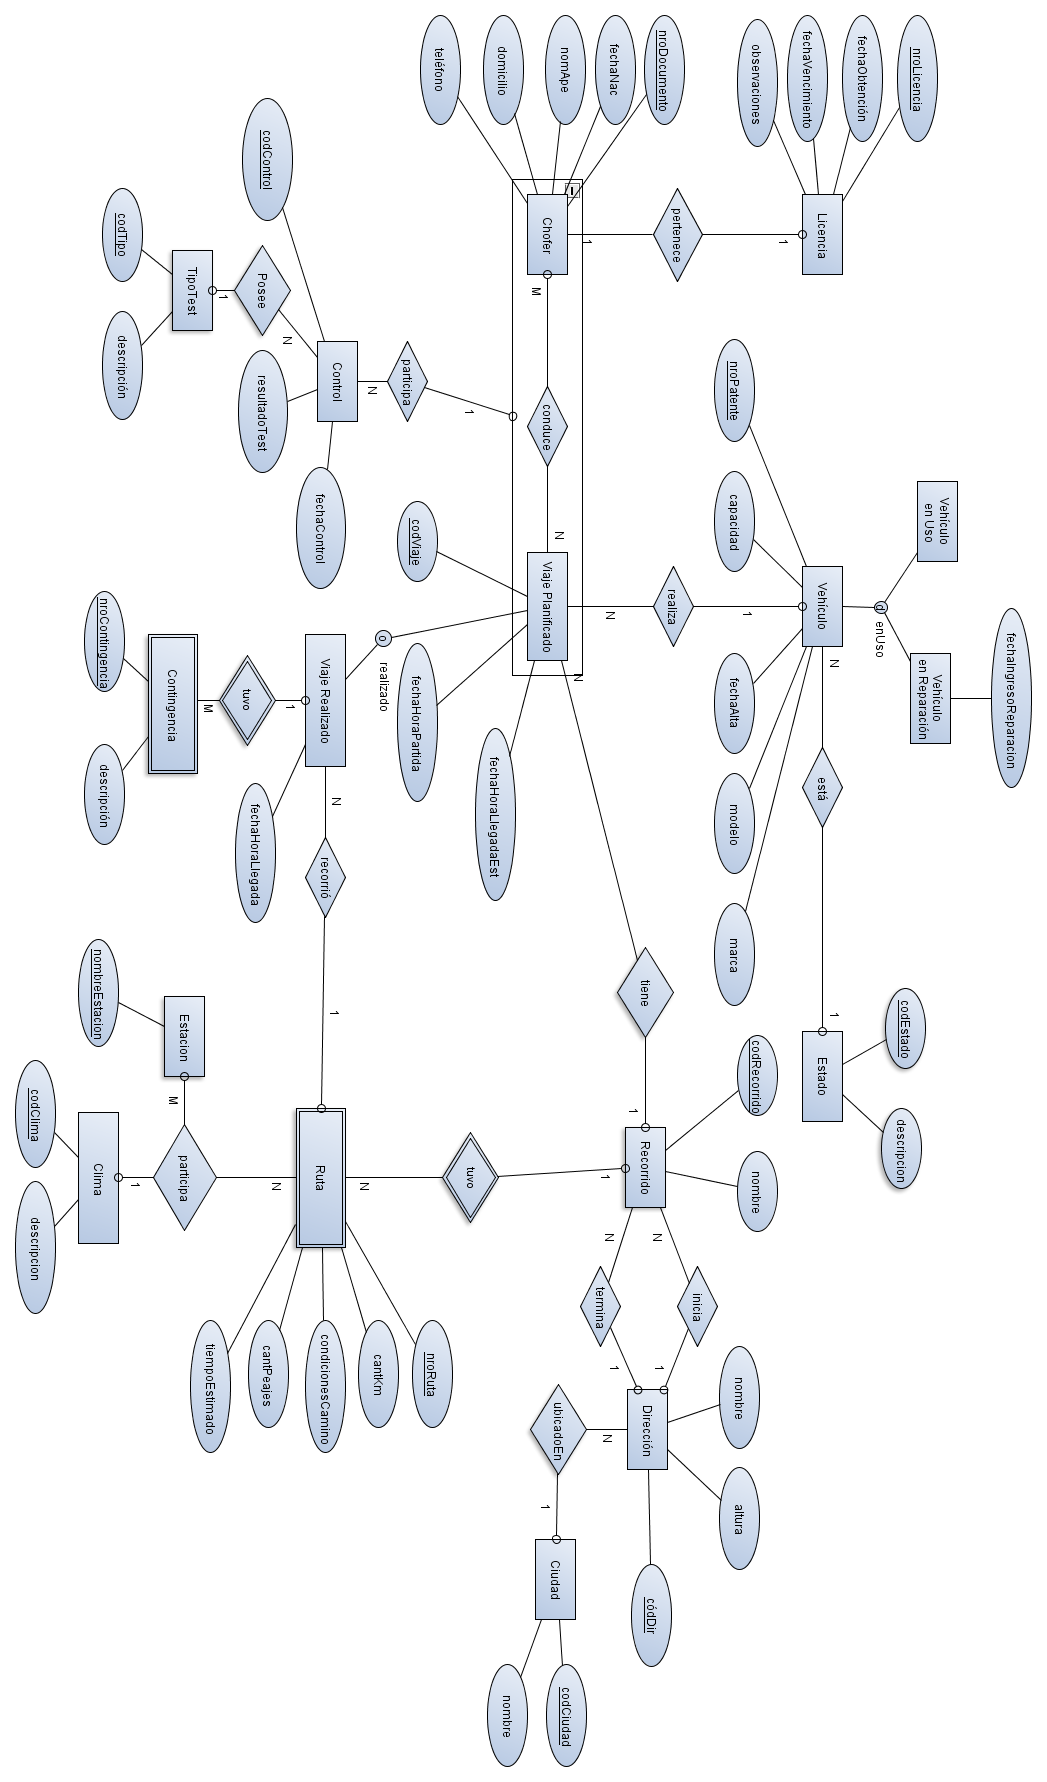
\includegraphics[height=0.95\textheight]{img/der.png}
\end{center}

\subsection{Restricciones}

\begin{enumerate}
	\item Dado 2 recorridos con distinto codigo, su origen y destino no pueden ser los mismos. Es decir, no puede haber dos recorridos ``iguales''con distinto c�digo. \label{MER1}
	\item Para todo recorrido, el origen no puede ser igual al destino \label{MER2}
	\item El recorrido de la ruta de todo viaje realizado debe ser igual al recorrido del viaje planificado.\label{MER3}
	\item Para todo recorrido que tiene un viaje planificado asociado, existe una ruta.\label{MER4}
	\item Para todo viaje la cantidad de conductores debe ser entre 1 y 3 y la fechaHoraLlegadaEst debe ser mayor a fechaHoraPartida.\label{MER5}
	\item Para todo viaje realizado la fechaHoraLlegada debe ser mayor a fechaHoraPartida.\label{MER6}
	\item Para todo viaje planificado que no esta realizado el vehiculo utilizado debe estar en uso.\label{MER7}	
	\item Para todo vehiculo en reparacion la fecha de ingreso es mayor a la fecha de alta.\label{MER8}
	\item Para toda licencia, la fecha de obtencion es menor a la fecha de vencimiento \label{MER9}
	\item Para todo chofer, la fecha de nacimiento es menor que la fecha de obtenci�n de su licencia \label{MER10}
	\item Para toda ruta, hay un �nico clima para todo per�odo definido \label{MER11}
	\item Para todo control, su fecha de realizaci�n debe ser anterior a la fecha de partida del viaje que se est� controlando  \label{MER12}
	\item La entidad Estaci�n puede tomar los valores, \textit{verano}, \textit{invierno}, \textit{oto�o} y \textit{primavera} \label{MER13}
\end{enumerate}
